\documentclass[a4paper]{article}
\usepackage[english]{babel}
\usepackage[utf8]{inputenc}
\usepackage{textcomp}
\usepackage{amsmath}
\usepackage{gensymb}
\usepackage{physics}
\usepackage{graphicx}
\usepackage[colorinlistoftodos]{todonotes}
\usepackage{xcolor}
\usepackage{array}
\usepackage{tabularx}
\usepackage{tikz}
\usepackage{framed}
\usepackage{xfrac}
\usepackage[most]{tcolorbox}
\usepackage{fix-cm}
\usepackage[margin=0.5in]{geometry}
\usetikzlibrary{quotes,angles}
\usetikzlibrary{decorations.pathreplacing}
\usetikzlibrary{calc}

\let\phi\varphi
\let\bf\textbf
\colorlet{shadecolor}{orange!15}
\def\centerarc[#1](#2)(#3:#4:#5){\draw[#1] ($(#2)+({#5*cos(#3)},{#5*sin(#3)})$) arc (#3:#4:#5)}
% Syntax: [draw options] (center) (initial angle:final angle:radius);

\title{Fixed-Axis Rotation}
\author{OpenStax University Physics Vol. 1}

\begin{document}
\setcounter{section}{10}
\maketitle
\subsection{Rotational Variables}
\noindent\bf{Angular Velocity}
\vspace{2mm}\\
Uniform circular motion is motion in a circle at constant speed, although this is the simplest case of rotational motion, it is used here to introduce rotational variables.\par
The figure shows a particle moving in a circle. Its position vector from the origin of the circle to the particle sweeps out the angle $\theta$, which increases in the counterclockwise direction as the particle moves along its path. The angle $\theta$ is called the angular position of the particle. As the particle moves, it traces an arc length $s$.
\begin{center}
    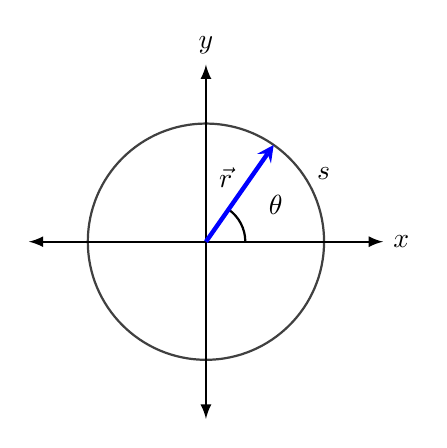
\begin{tikzpicture}[scale=1.5]
        %%% COORDINATES %%%
        \draw (0,0) coordinate (o);
        \draw ({cos(55)},{sin(55)}) coordinate (a);
        \draw ({cos(55)},0) coordinate (b);

        %%% AXES & CIRCLE %%%
        \draw[thick,draw=black!75] (0,0) circle (1);
        \draw[<->,thick,-latex] (0,0)--(1.5,0) node[right]{$x$};
        \draw[<->,thick,-latex] (0,0)--(0,1.5) node[above]{$y$};
        \draw[<->,thick,-latex] (0,0)--(-1.5,0);
        \draw[<->,thick,-latex] (0,0)--(0,-1.5);

        %%% POSITION VECTOR & ANGLE %%%
        \draw pic["$\theta$",draw=black,thick,-,angle eccentricity=2,angle radius=0.5cm]{angle=b--o--a};
        \draw[->,ultra thick,draw=blue,-stealth] (0,0)--node[left,xshift=0.5mm,yshift=2mm]{$\vec{r}$}({cos(55)},{sin(55)});

        \centerarc[red,very thick](0,0)(0:55:1);
        \node at ({1.15*cos(30)},{1.15*sin(30)}){$s$};
    \end{tikzpicture}
\end{center}
The angle is related to the radius of the circle and the arc length by 
\begin{equation}
    \theta = \frac{s}{r}
\end{equation}
\end{document}